\begin{figure*}[!t]\centering
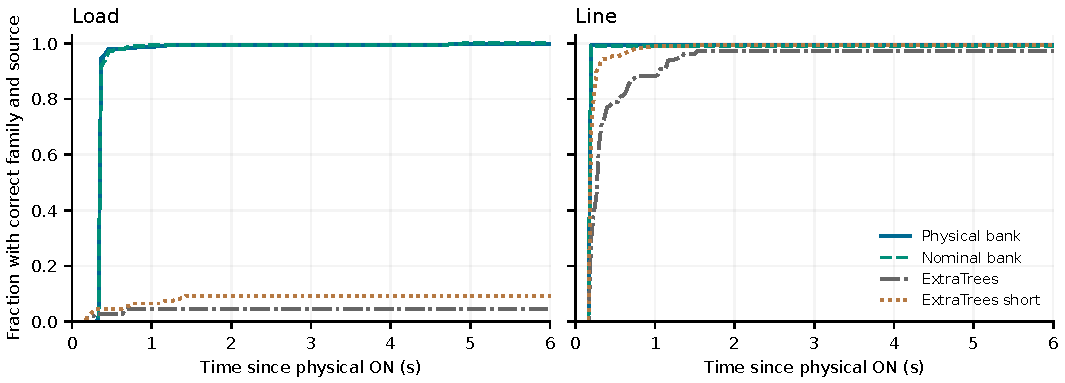
\includegraphics[width=.92\textwidth]{figures/generated/diagnosis_delay_distribution.pdf}
\caption{Distribution of correct diagnosis time, using all 324 replays per
true family in each denominator. An incorrect or absent diagnosis
contributes no mass, and late correct decisions are included, so the
curves differ from the before-OFF endpoint.}
\label{fig:diagnosis-time}\end{figure*}

\begin{figure*}[!t]\centering
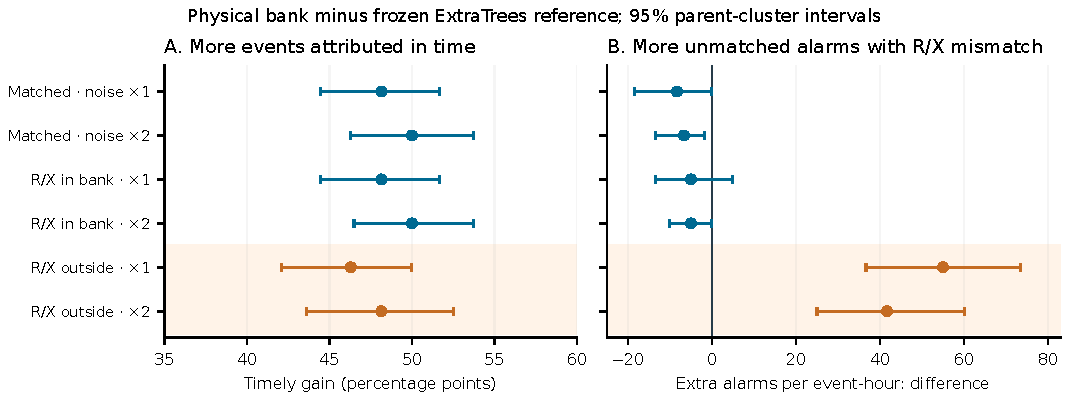
\includegraphics[width=.89\textwidth]{figures/generated/reader_c01_intervals.pdf}
\caption{Physical bank minus the ExtraTrees reference in the six paired
strata. Points and 95\% intervals come from 10{,}000 physical-parent
resamples. Left: percentage-point difference in timely attribution; right:
difference in unmatched alarms per monitored event-record hour (the 12-s
startup is excluded). Orange rows mark out-of-bank R/X conditions.}
\label{fig:c01-ci}\end{figure*}

\begin{figure*}[!t]\centering
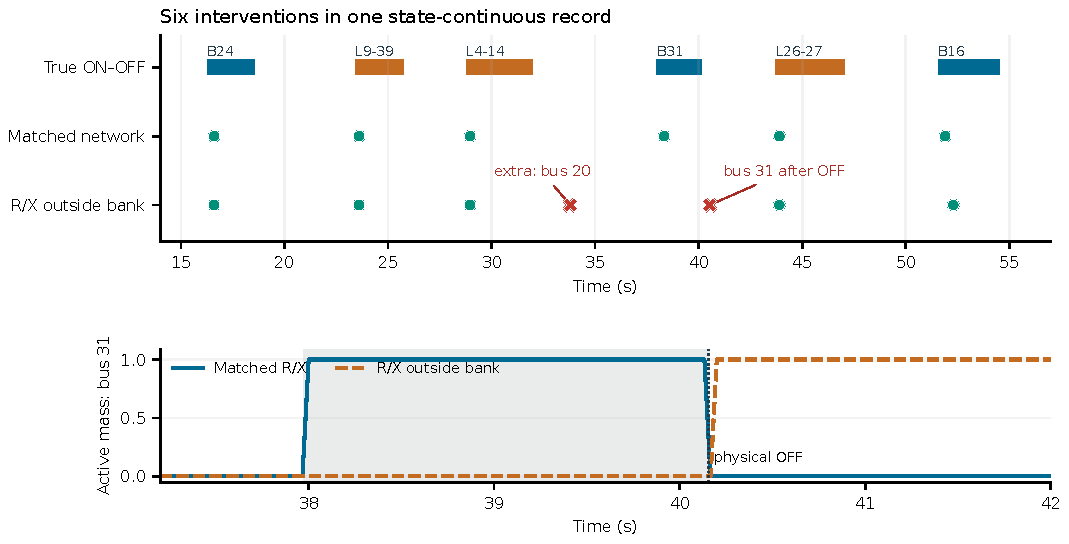
\includegraphics[width=.94\textwidth]{figures/generated/reader_episode_story.pdf}
\caption{One continuous development trajectory, shown for interpretation.
Top: physical ON--OFF intervals and emitted diagnoses under matched and
out-of-bank R/X. Bottom: bus-31 active mass with the true intervention
shaded. A diagnosis after OFF misses the timely endpoint even when it
identifies the source. True timing enters only this retrospective display.}
\label{fig:reader-story}\end{figure*}
